    Having looked at the $G$-Machine as a sequential abstract machine we can now
look at how graph reduction can occur on parallel architectures. The simplest
parallel variant would be a parallel $G$-Machine. It turns out that once a
sequential graph reduction has been accounted for there is not much to add in
order to provide facilities for parallel evaluation. If one were to use a shared
graph almost all communication could take place via that graph.

\begin{figure}[h]
  \centering
  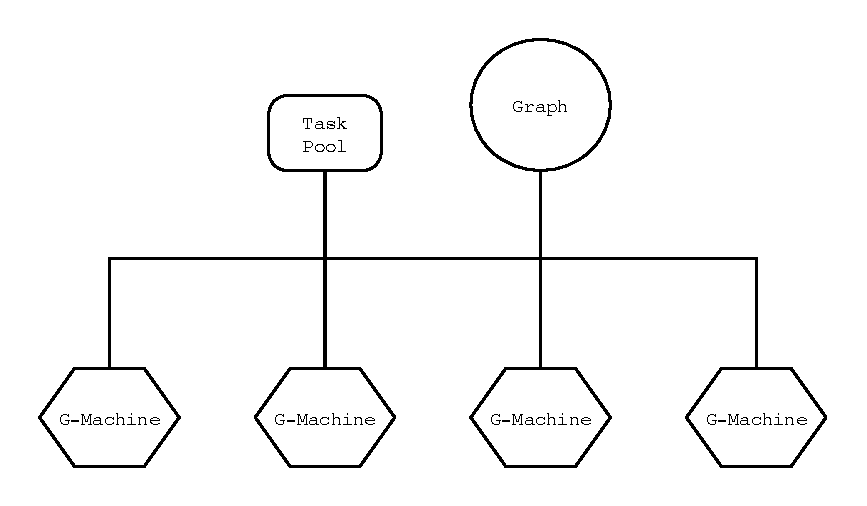
\includegraphics[scale=0.7]{Background/figures/simpleParallel.eps}
  \caption[Simple parallel graph reduction model]
   {A parallel G-Machine}
    \label{fig:simpleGMachine}
\end{figure}

The spark pool is where idle processors can look for subgraphs that have been
sparked off for evaluation. This simple-yet-functioning model is actually the
basis for the implementation described in chapter \ref{chap:platform}
\citep{PeytonJones:IFL}. This model is not specific to the $G$-Machine, but can
be used with any of the graph reduction machines, indeed GHC uses a similar
model that is extended with thread-local heaps \citep{marlow2009runtime}. A
worker thread allocates from its local heap, when a thread's heap has
overflowed the garbage collector stops \emph{all} running threads and moves local-heap data to
the shared heap.

 \subsection{$\langle \nu , G\rangle $-Machine}
    A departure from the stack-based approach of the G-Machine, here we have a
packet-based abstract machine \citep{vGMachine, Alice}.
    The packets (or frame as they are called in the
original paper) are similar to the closures we have seen for the STG-Machine
(although the $\langle \nu , G\rangle $-Machine was described and implemented
first \citep{vGMachine}). One difference is that on top of the code pointer and
pointer to its arguments, each node contains a dynamic pointer that points to the caller of
the expression the packet represents. Each node also contains a block of free `working
space' on each packet (we will see why in a moment).
The key difference is the way that the
$\langle \nu , G\rangle $-Machine deals with its stack.
As opposed to having a central stack, each packet has its own, using the free
space allocated with the creation of the packet as its local stack.
Therefore the stack for a task is always in
the heap with the task itself \citep{vGMachine}. This is in contrast to the standard
G-Machine, where the stack resides `in' the machine itself and the tasks use
that stack until they are blocked, at which point the task's stack is
transferred to the heap until the task is awoken.
    The $\langle \nu , G\rangle $-Machine avoids any complications of dealing
with the stack by distributing the stack amongst the graph. The stack frame at
any point in the graph is a accessed through the linked list of packets pointing
to their caller.
